\subsection{External links in privacy policies}
\label{sec:policy-links}


Companies may provide links to opt-out pages, industry organizations, or third-party partners that they share data with. Analyzing links found in the privacy policies may reveal trends in third-party data sharing and the effect of regulation on transparency.

To extract the links, we first parsed the policy's readable HTML source (i.e. source of the main article) using the Beautiful Soup Python library~\cite{beautifulsoup4}, and extracted the \texttt{href} attribute of each link (\texttt{<a>}) element. 
Using readable HTML sources allowed us to exclude links that were found in the footers, headers and sidebars of the privacy policies.
Next, we searched for a URL regular expression pattern in the policy texts to identify links that were not marked up, that is, included inline as plain text.
Using policy texts also allowed us to identify the links in the PDF privacy policies, which did not have associated HTML sources.

We then removed malformed or mistyped URLs by removing links that do not have a top level domain (TLD) in the IANA list of approved TLDs~\cite{iana-tld}. We also excluded the links having the same domain as the privacy policy snapshot.
% TODO: use also home domain to exclude first party links

Following these steps, we extracted 1,278,539 external links from 402,294 policy snapshots.
We found that 402,294 of the 910,546 (44.2\%) policy snapshots had at least one external link.
Overall, 63,308 of the 108,311 (58.5\%) websites had at least one external link in one of their policy snapshots in our dataset.


\begin{figure}[h]
\centering
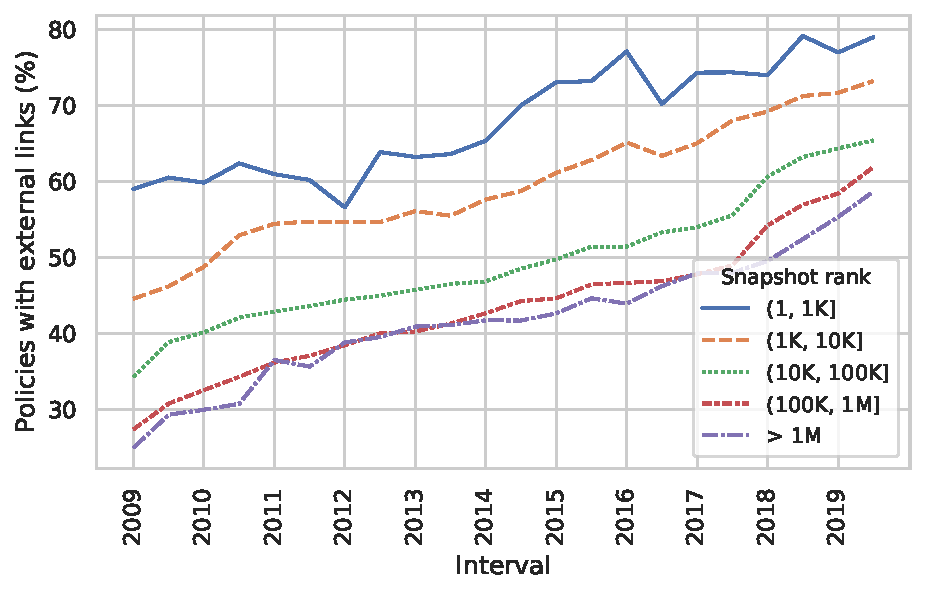
\includegraphics[width=0.99\columnwidth]{figures/lineplot_policies_with_external_links_pct.pdf}
\caption{Percentage of policies linking to one or more external domains.}
\label{fig:pct-policies-with-links}
\end{figure}


Figure~\ref{fig:pct-policies-with-links} shows that more recent policies and policies from more popular snapshots are more likely to link to external domains. Almost 80\% of the policies in the Alexa top 1K include one or more external links in the latest interval, compared to roughly 60\% of the snapshots in the 100K-1M rank range. 
Policies from less popular websites also show an upward trend: in the last ten years, the percentage of policies containing an external link doubled (from 31\% to 62\%) for snapshots that were ranked in the Alexa 100K-1M rank range.

We identify a similar trend in the number of distinct link domains, which may identify distinct third parties that policies link to. The average number of distinct domains policies link to increased more than three-fold (from 0.70 to 2.3) in the last ten years. %Figure~\ref{top-link-domains} shows 
We observe a steep increase after the introduction of the GDPR; the average number of distinct link domains increased by 80\% (1.3 to 2.3) in just two years, between the second half of 2017 and 2019.
The highest number of distinct link domains in a privacy policy snapshot was from an online course website (alison.com). The snapshot, which appeared in the second half of 2018, includes links to 329 distinct third party partners.


\begin{table}[]
\centering
\resizebox{0.95\columnwidth}{!}{%
\begin{tabular}{@{}lrl@{}}
\toprule
\textbf{URL} & \textbf{Num. of sites} & \textbf{Purpose} \\ \midrule
google.com/privacy\_ads.html & 11,324 (17.9\%) & Privacy/ToS \\
networkadvertising.org/managing/opt\_out.asp & 9,290 (14.7\%) & Opt-out \\
tools.google.com/dlpage/gaoptout & 5,645 (8.9\%) & Opt-out* \\
aboutads.info/choices & 5,287 (8.4\%) & Opt-out \\
networkadvertising.org & 3,858 (6.1\%) & Industry org. \\
networkadvertising.org/choices & 3,692 (5.8\%) & Opt-out \\
allaboutcookies.org & 3,669 (5.8\%) & Help page \\
aboutads.info & 2,659 (4.2\%) & Opt-out \\
export.gov/safeharbor & 2,565 (4.1\%) & Safe Harbor \\ \bottomrule
\end{tabular}%
}
\caption{Ten most common external links found in privacy policies.\\
*: Google Analytics Opt-out Browser Add-on page.}
\label{top-links}
\end{table}


Table~\ref{top-links} shows the ten most common pages privacy policies link to by distinct websites.
Google’s advertisement privacy and terms of service page is linked from 69,998 policy snapshots that belong
to 11,324 distinct websites (17.9\% of all websites in the dataset).
Five of the ten entries in the table are links to opt-out related pages; including ad industry opt-out pages, and Google Analytics Opt-out Browser Add-on, which was released in 2010~\cite{GA-opt-out}.
% Finally, the tenth most link is to Safe Harbor.

\subsubsection{Links to tracker domains}

Next, we investigate privacy policy links to tracking companies.

We use external sources to determine whether a link belongs to a tracker or not. We use three adblocking lists: Disconnect~\cite{disconnectme2020May}, EasyList~\cite{EasyList} and EasyPrivacy~\cite{EasyPrivacy} as they are very commonly used to detect ads and trackers by millions of users everyday.
EasyList and EasyPrivacy are used by popular adblocking extensions Adblock Plus and uBlockOrigin. Disconnect’s list is used by Firefox browser’s Enhanced Tracking Protection mode to detect and block trackers~\cite{Firefox-TPM}.
In addition to the adblocking lists, we used member lists of NAI~\cite{NAI-member-list} and DAA~\cite{DAA-member-list}, two digital advertising industry organizations. We flagged a link as a ``tracking'', if it is flagged as a tracker by any of these sources.

We found that 220,228 of the 910,546 snapshots (24\%) have at least one link categorized as tracking.
Since websites have multiple snapshots in the sample, we first take distinct (website, link URL) pairs.
Of these 327,862 distinct pairs, 40.5\% of the links were categorized as tracking.

The top tracker domains linked from the privacy policies are given in Table~\ref{tab:top-ten-tracker}.
\gnote{add comments}

%The most common domains policies link to include tracking companies (e.g., Google, Facebook), online behavioral advertising (OBA) opt-out pages (aboutads.info) and ad industry organizations (networkadvertising.org) (Table~\ref{top-link-domains}). The list also includes two .gov domains, namely export.gov (which hosted the Safe Harbor page) and privacyshield.gov, two frameworks for exchange of personal data between the US and the EU.


\begin{itemize}
    \item Do privacy regulations require linking to embedded third parties?
\end{itemize}

\begin{comment}

\begin{figure}[h]
\centering
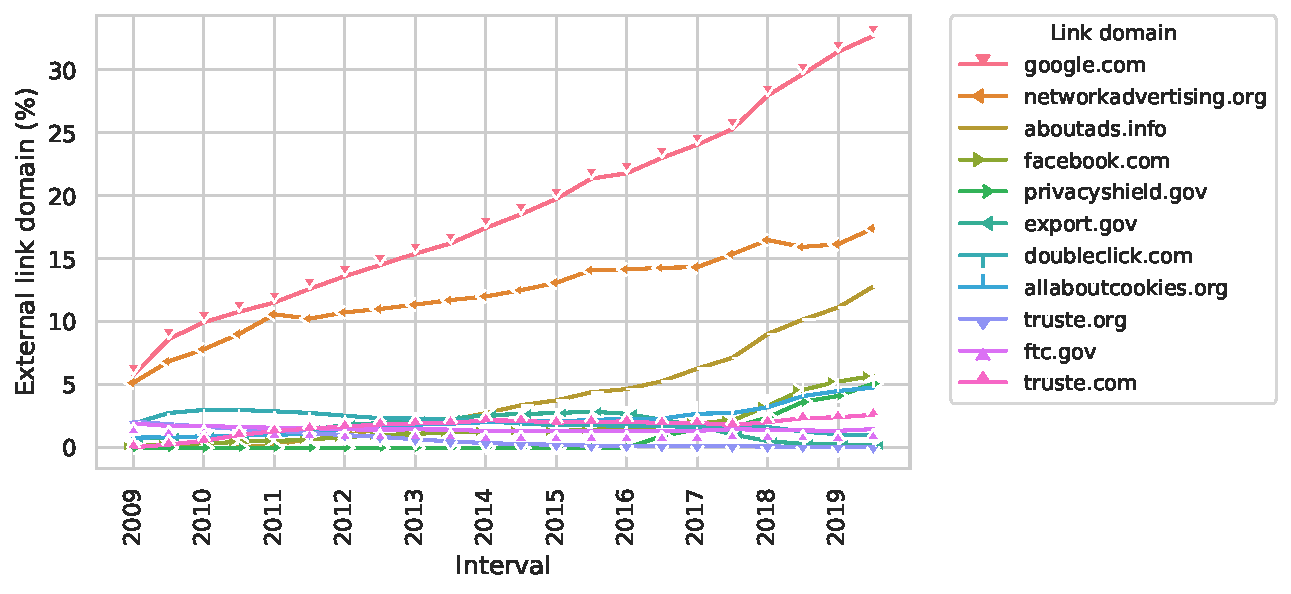
\includegraphics[width=0.99\columnwidth]{figures/top5_link_domains_2009.pdf}
\caption{Link domains that were in the top 5 most common.}
\label{fig:top-5-link-domain}
\end{figure}
\end{comment}


\begin{comment}

\begin{figure}[t]
\centering
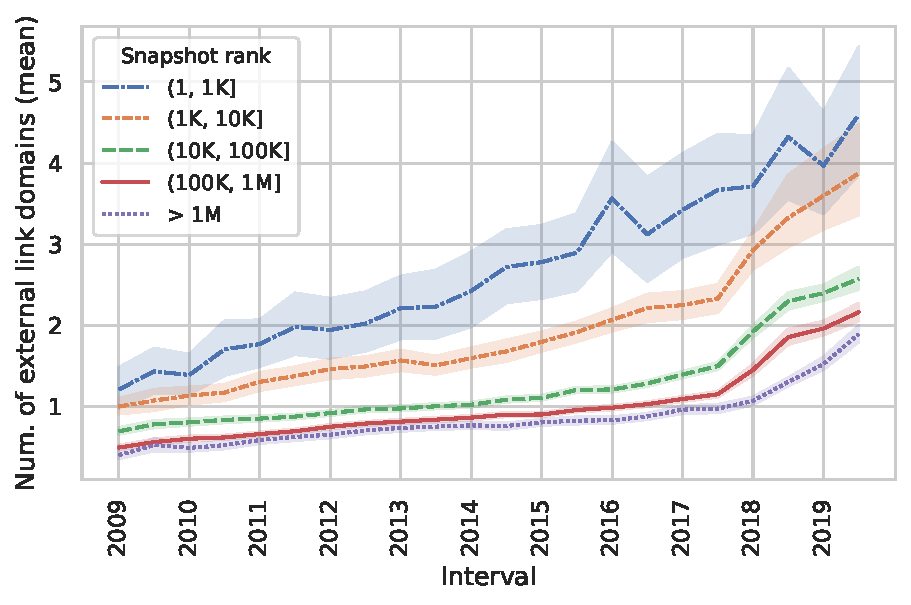
\includegraphics[width=0.99\columnwidth]{figures/lineplot_num_of_external_link_domains_mean.pdf}
\caption{Average number of external domains privacy policies link to.}
\label{fig:num-distinct-ext-domain}
\end{figure}


\begin{figure}[t]
\centering
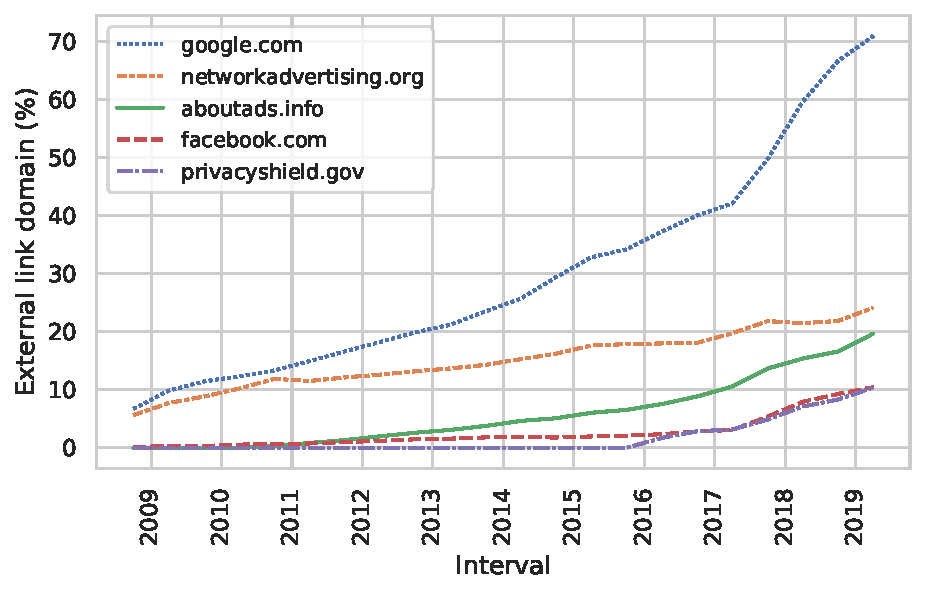
\includegraphics[width=0.99\columnwidth]{figures/lineplot_link_domain_2009_onwards.pdf}
\caption{Top external link domains found in the privacy policies}
\label{fig:top-external-link-domain}
\end{figure}


\begin{figure}[t]
\centering
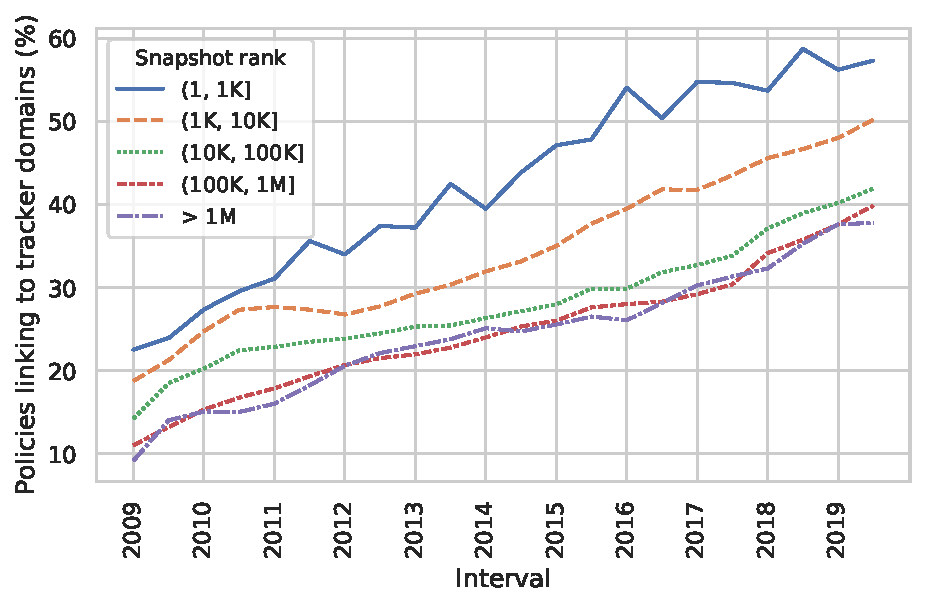
\includegraphics[width=0.99\columnwidth]{figures/lineplot_policies_linking_to_tracker_domains_pct.pdf}
\caption{Percentage of policies linking to one or more tracker domains.}
\label{fig:pct-tracker-link}
\end{figure}
\end{comment}


\begin{comment}
\begin{table}[]
\centering
\begin{tabular}{@{}lrr@{}}
\toprule
\textbf{Domain}        & \textbf{Num. of sites} & \textbf{\%} \\ \midrule
google.com             & 29311                  & 46.3        \\
networkadvertising.org & 18248                  & 28.8        \\
aboutads.info          & 8313                   & 13.1        \\
allaboutcookies.org    & 4245                   & 6.7         \\
facebook.com           & 4235                   & 6.7         \\
truste.com             & 2883                   & 4.6         \\
microsoft.com          & 2787                   & 4.4         \\
export.gov             & 2780                   & 4.4         \\
doubleclick.com        & 2642                   & 4.2         \\
privacyshield.gov      & 2456                   & 3.9         \\ \bottomrule
\end{tabular}
\caption{Ten most common external domains privacy policies link to.}
\label{top-link-domains}
\end{table}
\end{comment}


\begin{table}[]
\centering
\resizebox{0.55\columnwidth}{!} \\ \midrule
google.com & 29,311 & 72.4 \\
facebook.com & 4,235 & 10.5 \\
truste.com & 2,883 & 7.1 \\
microsoft.com & 2,787 & 6.9 \\
doubleclick.com & 2,642 & 6.5 \\
twitter.com & 2,397 & 5.9 \\
adobe.com & 1,943 & 4.8 \\
yahoo.com & 1,125 & 2.8 \\
automattic.com & 1,042 & 2.6 \\
amazon.com & 995 & 2.5 \\ \bottomrule
\end{tabular}
}
\caption{Top ten tracker domains linked from privacy policies.}
\label{tab:top-ten-tracker}
\end{table}
